% ============================================================
% Chapitre 4 : Proprietes des Estimateurs
% ============================================================
\chapter{Propri\'et\'es des Estimateurs --- Biais, Convergence, Efficacit\'e}
\label{ch:proprietes}

\begin{center}
\textit{<<~Un bon estimateur doit viser juste et ne pas trop se disperser.~>>}
\end{center}

% ------------------------------------------------------------
\section{Exemple motivant}
% ------------------------------------------------------------

Deux tireurs visent une cible. Le premier touche en moyenne le centre mais ses tirs sont dispers\'es. Le second groupe ses tirs mais d\'ecal\'es syst\'ematiquement \`a droite. Lequel est <<~meilleur~>> ? Cette question se pose exactement pour les estimateurs : il faut comprendre le \textbf{biais}, la \textbf{variance} et leur compromis.

% ------------------------------------------------------------
\section{Biais d'un estimateur}
% ------------------------------------------------------------

\begin{definition}[Biais]
\index{biais}
Le \textbf{biais} de l'estimateur $\thetahat$ de $\theta$ est :
\[
\Biais(\thetahat) = \E_\theta[\thetahat] - \theta.
\]
$\thetahat$ est dit \textbf{sans biais} si $\Biais(\thetahat)=0$ pour tout $\theta\in\Theta$, i.e.\ $\E_\theta[\thetahat]=\theta$.
\end{definition}

\begin{exemple}
$X_1,\ldots,X_n\iid$ avec $\E[X_i]=\mu$. Alors $\xbar$ est sans biais pour $\mu$ : $\E[\xbar]=\mu$.
\end{exemple}

\begin{proposition}
$S^2=\frac{1}{n-1}\sum_{i=1}^n(X_i-\xbar)^2$ est un estimateur sans biais de $\sigma^2$.
\end{proposition}

\begin{proof}
\begin{align*}
\sum_{i=1}^n(X_i-\xbar)^2 &= \sum_{i=1}^n X_i^2 - n\xbar^2.
\end{align*}
Or $\E[X_i^2]=\Var(X_i)+(\E[X_i])^2=\sigma^2+\mu^2$ et $\E[\xbar^2]=\Var(\xbar)+\mu^2=\frac{\sigma^2}{n}+\mu^2$. Donc :
\[
\E\!\left[\sum(X_i-\xbar)^2\right] = n(\sigma^2+\mu^2)-n\left(\frac{\sigma^2}{n}+\mu^2\right) = (n-1)\sigma^2.
\]
D'o\`u $\E[S^2]=\sigma^2$.
\end{proof}

\begin{definition}[Biais asymptotique]
$\thetahat_n$ est \textbf{asymptotiquement sans biais} si $\Biais(\thetahat_n)\to 0$ quand $n\to\infty$.
\end{definition}

% ------------------------------------------------------------
\section{Erreur quadratique moyenne}
% ------------------------------------------------------------

\begin{definition}[EQM / MSE]
\index{EQM}\index{erreur quadratique moyenne}
L'\textbf{erreur quadratique moyenne} est :
\[
\EQM(\thetahat) = \E_\theta[(\thetahat-\theta)^2].
\]
\end{definition}

\begin{theoreme}[D\'ecomposition biais-variance]
\label{thm:biais-variance}
\[
\EQM(\thetahat) = \Var(\thetahat) + \bigl[\Biais(\thetahat)\bigr]^2.
\]
\end{theoreme}

\begin{proof}
Posons $b=\E[\thetahat]-\theta$. Alors :
\begin{align*}
\EQM(\thetahat) &= \E[(\thetahat-\theta)^2] = \E[(\thetahat-\E[\thetahat]+b)^2] \\
&= \E[(\thetahat-\E[\thetahat])^2] + 2b\,\E[\thetahat-\E[\thetahat]] + b^2 = \Var(\thetahat)+b^2. \qedhere
\end{align*}
\end{proof}

\begin{intuition}
L'EQM combine deux sources d'erreur. Un estimateur biais\'e peut avoir un EQM plus faible qu'un estimateur sans biais si sa variance est suffisamment r\'eduite. C'est le \textbf{compromis biais-variance}, fondamental en apprentissage statistique.
\end{intuition}

\begin{center}
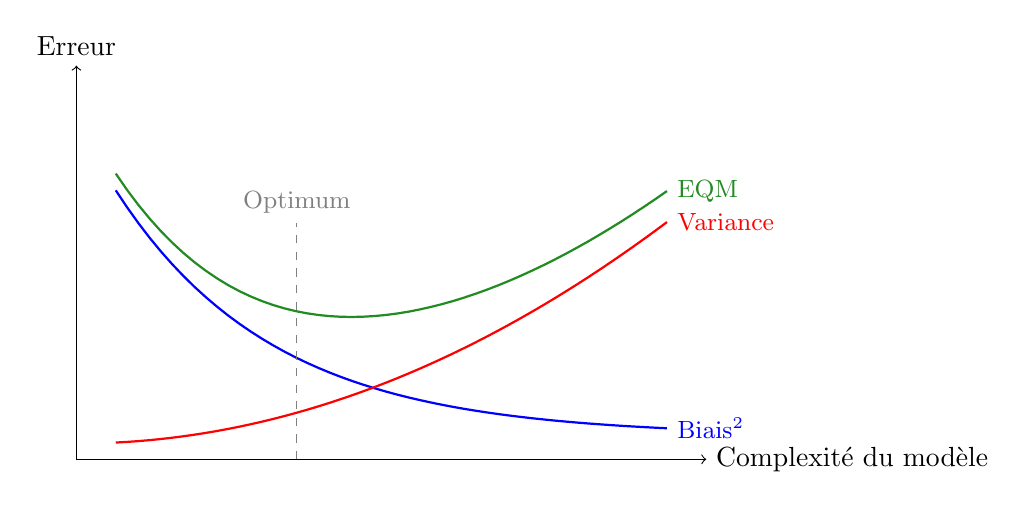
\begin{tikzpicture}
% Bias-variance tradeoff illustration
\draw[->] (0,0) -- (8,0) node[right] {Complexit\'e du mod\`ele};
\draw[->] (0,0) -- (0,5) node[above] {Erreur};
\draw[thick,blue,domain=0.5:7.5,samples=50] plot (\x, {4*exp(-0.5*\x)+0.3}) node[right] {\small Biais$^2$};
\draw[thick,red,domain=0.5:7.5,samples=50] plot (\x, {0.05*\x*\x+0.2}) node[right] {\small Variance};
\draw[thick,ForestGreen,domain=0.5:7.5,samples=50] plot (\x, {4*exp(-0.5*\x)+0.05*\x*\x+0.5}) node[right] {\small EQM};
\draw[dashed,gray] (2.8,0) -- (2.8,3) node[above] {\small Optimum};
\end{tikzpicture}
\end{center}

% ------------------------------------------------------------
\section{Convergence (consistance)}
% ------------------------------------------------------------

\begin{definition}[Estimateur convergent (consistant)]
\index{convergence}\index{consistance}
$\thetahat_n$ est \textbf{convergent} (ou consistant) pour $\theta$ si :
\[
\thetahat_n \xrightarrow{\Prob} \theta \quad (n\to\infty),
\]
c'est-\`a-dire $\forall\varepsilon>0$, $\Prob(|\thetahat_n-\theta|>\varepsilon)\to 0$.
\end{definition}

\begin{proposition}[Condition suffisante]
\label{prop:consistance}
Si $\Biais(\thetahat_n)\to 0$ et $\Var(\thetahat_n)\to 0$ quand $n\to\infty$, alors $\thetahat_n$ est convergent.
\end{proposition}

\begin{proof}
Par l'in\'egalit\'e de Tchebychev :
\[
\Prob(|\thetahat_n-\theta|>\varepsilon) \leq \frac{\EQM(\thetahat_n)}{\varepsilon^2} = \frac{\Var(\thetahat_n)+\Biais^2(\thetahat_n)}{\varepsilon^2} \to 0. \qedhere
\]
\end{proof}

\begin{exemple}
$\xbar$ est convergent pour $\mu$ : $\Biais(\xbar)=0$ et $\Var(\xbar)=\sigma^2/n\to 0$.
\end{exemple}

% ------------------------------------------------------------
\section{Efficacit\'e et borne de Cram\'er--Rao}
% ------------------------------------------------------------

\begin{definition}[Score et conditions de r\'egularit\'e]
\index{score}
Le \textbf{score} est $S(\theta)=\frac{\partial}{\partial\theta}\ln f(X;\theta)$. Les conditions de r\'egularit\'e exigent que :
\begin{enumerate}
\item Le support de $f(\cdot;\theta)$ ne d\'epend pas de $\theta$.
\item On peut d\'eriver sous le signe int\'egrale.
\item $0 < I(\theta) < \infty$.
\end{enumerate}
\end{definition}

\begin{theoreme}[In\'egalit\'e de Cram\'er--Rao]
\index{Cramer-Rao@Cram\'er--Rao}
\label{thm:cramer-rao}
Sous les conditions de r\'egularit\'e, pour tout estimateur sans biais $\thetahat$ de $g(\theta)$ :
\[
\Var_\theta(\thetahat) \geq \frac{[g'(\theta)]^2}{nI(\theta)}.
\]
En particulier, si $\thetahat$ est sans biais pour $\theta$ ($g=\mathrm{id}$) :
\[
\Var_\theta(\thetahat) \geq \frac{1}{nI(\theta)}.
\]
\end{theoreme}

\begin{proof}
Par l'in\'egalit\'e de Cauchy--Schwarz. Posons $U=\thetahat$ et $V=\sum_{i=1}^n\frac{\partial}{\partial\theta}\ln f(X_i;\theta)$ (score total). On sait que $\E[V]=0$ (d\'erivation sous l'int\'egrale) et $\Var(V)=nI(\theta)$.

Comme $\thetahat$ est sans biais pour $g(\theta)$ : $\E_\theta[\thetahat]=g(\theta)$. En d\'erivant :
\[
g'(\theta) = \frac{\partial}{\partial\theta}\int \thetahat \prod f(x_i;\theta)\,d\mathbf{x} = \E_\theta[\thetahat\cdot V] = \Cov(\thetahat,V).
\]
Par Cauchy--Schwarz : $[g'(\theta)]^2 = [\Cov(\thetahat,V)]^2 \leq \Var(\thetahat)\cdot\Var(V) = \Var(\thetahat)\cdot nI(\theta)$.
\end{proof}

\begin{definition}[Estimateur efficace]
\index{efficacite@efficacit\'e}
$\thetahat$ est \textbf{efficace} s'il atteint la borne de Cram\'er--Rao : $\Var(\thetahat)=\frac{1}{nI(\theta)}$.
\end{definition}

\begin{exemple}
Pour $X_i\iid\mathcal{N}(\mu,\sigma^2)$ ($\sigma^2$ connu) : $I(\mu)=1/\sigma^2$ et $\Var(\xbar)=\sigma^2/n=1/(nI(\mu))$. Donc $\xbar$ est \textbf{efficace}.
\end{exemple}

\begin{definition}[Efficacit\'e relative]
L'\textbf{efficacit\'e relative} de $\thetahat_1$ par rapport \`a $\thetahat_2$ est :
\[
e(\thetahat_1,\thetahat_2) = \frac{\Var(\thetahat_2)}{\Var(\thetahat_1)}.
\]
Si $e>1$, $\thetahat_1$ est plus efficace.
\end{definition}

% ------------------------------------------------------------
\section{Estimateur UMVUE et th\'eor\`eme de Rao--Blackwell}
% ------------------------------------------------------------

\begin{definition}[UMVUE]
\index{UMVUE}
Un estimateur sans biais $\thetahat^*$ de $g(\theta)$ est \textbf{UMVUE} (Uniformly Minimum Variance Unbiased Estimator) si pour tout autre estimateur sans biais $\thetahat$ de $g(\theta)$ :
\[
\Var_\theta(\thetahat^*) \leq \Var_\theta(\thetahat) \quad \forall\theta\in\Theta.
\]
\end{definition}

\begin{theoreme}[Rao--Blackwell]
\index{Rao--Blackwell}
Soit $\thetahat$ un estimateur sans biais de $g(\theta)$ et $T$ une statistique exhaustive. Alors $\thetahat^* = \E[\thetahat\mid T]$ est :
\begin{enumerate}
\item Sans biais pour $g(\theta)$,
\item $\Var(\thetahat^*)\leq\Var(\thetahat)$, avec \'egalit\'e ssi $\thetahat$ est d\'ej\`a fonction de $T$.
\end{enumerate}
\end{theoreme}

\begin{proof}
(1) $\E[\thetahat^*]=\E[\E[\thetahat\mid T]]=\E[\thetahat]=g(\theta)$ (tour de l'esp\'erance).

(2) Par la formule de d\'ecomposition de la variance :
\[
\Var(\thetahat) = \E[\Var(\thetahat\mid T)] + \Var(\E[\thetahat\mid T]) = \E[\Var(\thetahat\mid T)] + \Var(\thetahat^*).
\]
Comme $\E[\Var(\thetahat\mid T)]\geq 0$, on a $\Var(\thetahat)\geq\Var(\thetahat^*)$.
\end{proof}

\begin{theoreme}[Lehmann--Scheff\'e]
\index{Lehmann--Scheff\'e}
Si $T$ est exhaustive et \textbf{compl\`ete}, alors tout estimateur sans biais fonction de $T$ est UMVUE.
\end{theoreme}

% ------------------------------------------------------------
\section{Impl\'ementation Python}
% ------------------------------------------------------------

\begin{python}
\begin{minted}{python}
import numpy as np
import matplotlib.pyplot as plt

np.random.seed(42)

# --- Comparaison biais et EQM de deux estimateurs de sigma^2 ---
mu_true, sigma2_true = 0, 4
n = 10
n_sim = 50000

estimates_biased = []   # diviseur n (EMV)
estimates_unbiased = []  # diviseur n-1

for _ in range(n_sim):
    sample = np.random.normal(mu_true, np.sqrt(sigma2_true), n)
    estimates_biased.append(np.var(sample, ddof=0))
    estimates_unbiased.append(np.var(sample, ddof=1))

estimates_biased = np.array(estimates_biased)
estimates_unbiased = np.array(estimates_unbiased)

print("=== Estimateur EMV (diviseur n) ===")
print(f"  E[hat_sigma^2] = {np.mean(estimates_biased):.4f} (biais = "
      f"{np.mean(estimates_biased) - sigma2_true:.4f})")
print(f"  Var = {np.var(estimates_biased):.4f}")
print(f"  EQM = {np.mean((estimates_biased - sigma2_true)**2):.4f}")

print("\n=== Estimateur S^2 (diviseur n-1) ===")
print(f"  E[S^2] = {np.mean(estimates_unbiased):.4f} (biais = "
      f"{np.mean(estimates_unbiased) - sigma2_true:.4f})")
print(f"  Var = {np.var(estimates_unbiased):.4f}")
print(f"  EQM = {np.mean((estimates_unbiased - sigma2_true)**2):.4f}")

# --- Borne de Cramer-Rao ---
# Pour N(mu, sigma^2=4 connu) : I(mu) = 1/sigma^2 = 0.25
# Borne CR pour n obs : 1/(n*I) = sigma^2/n
print(f"\nBorne de Cramer-Rao pour mu: {sigma2_true/n:.4f}")
print(f"Variance empirique de Xbar:  {np.var([np.mean(np.random.normal(0,2,n)) for _ in range(n_sim)]):.4f}")

# --- Visualisation ---
fig, ax = plt.subplots(figsize=(8, 5))
ax.hist(estimates_biased, bins=50, alpha=0.5, density=True, label='EMV (n)')
ax.hist(estimates_unbiased, bins=50, alpha=0.5, density=True, label='$S^2$ (n-1)')
ax.axvline(sigma2_true, color='red', lw=2, label=f'$\\sigma^2={sigma2_true}$')
ax.set_xlabel(r'$\hat{\sigma}^2$')
ax.set_ylabel('Densite')
ax.set_title(f'Distribution des estimateurs de $\\sigma^2$ (n={n})')
ax.legend()
plt.savefig("ch04_biais_variance.pdf")
plt.show()
\end{minted}
\end{python}

% ------------------------------------------------------------
\section{Exercices}
% ------------------------------------------------------------

\begin{exercice}[$\star$ -- Biais]
Soit $X_1,\ldots,X_n\iid\mathcal{E}(\lambda)$. L'estimateur $\hat{\lambda}=1/\xbar$ est-il sans biais pour $\lambda$ ? (Indication : \'etudier la loi de $n\xbar$.)
\end{exercice}

\begin{exercice}[$\star\star$ -- Cram\'er--Rao]
\begin{enumerate}
\item Calculer la borne de CR pour l'estimation sans biais de $p$ dans le mod\`ele $\mathcal{B}(1,p)$.
\item Montrer que $\xbar$ atteint cette borne.
\item En d\'eduire que $\xbar$ est UMVUE pour $p$.
\end{enumerate}
\end{exercice}

\begin{exercice}[$\star\star$ -- Rao--Blackwell]
Soit $X_1,\ldots,X_n\iid\mathcal{P}(\lambda)$. On consid\`ere l'estimateur $\thetahat=\mathbf{1}_{X_1=0}$ de $g(\lambda)=e^{-\lambda}=\Prob(X=0)$.
\begin{enumerate}
\item V\'erifier que $\thetahat$ est sans biais.
\item $T=\sum X_i$ est exhaustive pour $\lambda$. Calculer $\thetahat^*=\E[\thetahat\mid T]$.
\item Comparer $\Var(\thetahat)$ et $\Var(\thetahat^*)$.
\end{enumerate}
\end{exercice}

\begin{exercice}[$\star\star$ -- Compromis biais-variance]
Soit $X_1,\ldots,X_n\iid\mathcal{N}(\mu,\sigma^2)$. On consid\`ere l'estimateur $\thetahat_c = c\cdot S^2$ de $\sigma^2$ pour $c>0$.
\begin{enumerate}
\item Calculer le biais et l'EQM de $\thetahat_c$ en fonction de $c$.
\item Trouver la valeur $c^*$ qui minimise l'EQM. Est-ce $c=1/(n-1)$ ?
\end{enumerate}
\end{exercice}

\begin{exercice}[$\star\star\star$ -- Projet : efficacit\'e par simulation]
Pour la loi de Poisson $\mathcal{P}(\lambda)$ avec $\lambda=3$ :
\begin{enumerate}
\item V\'erifier num\'eriquement que $\xbar$ est efficace (atteint la borne CR).
\item Comparer par simulation l'EQM de $\xbar$, de la m\'ediane et de la variance empirique comme estimateurs de $\lambda$.
\item Tracer l'efficacit\'e relative en fonction de $n$.
\end{enumerate}
\end{exercice}

% ------------------------------------------------------------
\begin{formules}
\begin{align*}
\Biais(\thetahat) &= \E[\thetahat]-\theta \\
\EQM(\thetahat) &= \Var(\thetahat)+[\Biais(\thetahat)]^2 \\
\text{Cram\'er--Rao} &: \Var(\thetahat)\geq \frac{[g'(\theta)]^2}{nI(\theta)} \\
\text{Rao--Blackwell} &: \thetahat^*=\E[\thetahat\mid T],\;\Var(\thetahat^*)\leq\Var(\thetahat)
\end{align*}
Consistance : $\Biais\to 0$ et $\Var\to 0 \implies \thetahat\xrightarrow{\Prob}\theta$.
\end{formules}
